\section{Semaine 17 (03/02-07/02) }

\e{Notions abordées :}
\begin{itemize}
	\item Thermodynamique de MPSI.
	\item Systèmes thermodynamiques en écoulement.
\end{itemize}

\subsection{Questions de cours :}
\begin{enumerate}
	\item Énoncer la loi de Laplace ainsi que ses conditions de validité. La démontrer.
	\item Énoncer le premier principe pour un système ouvert. Quelle hypothèse importante a-t-elle été utilisée ?
	\item Dessiner l'allure typique du diagramme $(\ln P, h)$ pour un équilibre diphasique. Dessiner l'allure d'une isotherme. 
\end{enumerate}

\subsection{Exercice 1 : Machine frigorifique à fluide idéal}

Un fluide est utilisé dans une machine frigorifique de type pompe à chaleur, chargée de prélever de l'énergie thermique à l'eau d'un lac formant un thermostat et d'en restituer à l'air d'une pièce ou à l'eau d'une piscine.

Le fluide caloporteur est supposé idéal, en ce sens qu'il est un corps pur, se comporte comme un gaz parfait à l'état de vapeur, de rapport de capacités thermiques $\gamma$ et qu'il est non visqueux, incompressible et indilatable à l'état liquide, de capacité thermique massique $c_l$. On note $M$ sa masse molaire et $\Delta_{vap}h$ l'enthalpie molaire de vaporisation supposée indépendante de la température. 

Le fluide au point de rosée en A $(P_A, T_A)$ subit une compression adiabatique réversible jusqu'au point B $(P_B, T_B)$ à l'état de vapeur sèche. Il subit alors un refroidissement puis une liquéfaction isobares jusqu'au point d'ébullition C $(P_C, T_C)$. Il subit une détente isenthalpique jusqu'au point D diphasé $(P_D, T_D)$ et revient au point A par une vaporisation isobare.

On suppose les variations d'énergies potentielle et cinétique négligeables devant les variations d'enthalpie.

\begin{enumerate}
	\item Tracer l'allure du cycle dans un diagramme  $(\ln P, h)$.
	\item Donner la valeur de la température $T_D$ et calculer $T_B$.
	\item Donner les valeurs des titres massiques en vapeur $x_A$ et $x_C$. Calculer $x_D$ en décomposant judicieusement la transformation $(CD)$.
	\item Définir l'énergie coûteuse et l'énergie utile. 
	\item Déterminer l'énergie utile en décomposant judicieusement la transformation $(BC)$. 
	\item Déterminer l'énergie coûteuse.
	\item En déduire l'efficacité de la pompe à chaleur. Commenter.
\end{enumerate}

\e{Données :}
\begin{itemize}
	\item $\gamma = \SI{1.40}{}$, $M = \SI{50.0e-3}{kg\per\mol}$, $c_l = \SI{2.00e3}{\joule\per\kelvin\per\kilogram}$.
	\item $P_B = 3P_A$.
	\item $T_A = \SI{280}{K}$, $T_C = \SI{320}{K}$.
	\item $\Delta_{vap}h(\SI{320}{K}) = \SI{1.43e5}{\joule\per\kilogram}$.
\end{itemize}

\e{Réponses :}
\begin{enumerate}
	\item -
	\item $T_D = \SI{280}{K}$. $T_B = \SI{383}{K}$.
	\item $x_A = 1$, $x_C = 0$, $x_D = 0.40$.
	\item -
	\item $\SI{1.80e5}{\joule\per\kilogram}$
	\item $\SI{0.60e5}{\joule\per\kilogram}$
	\item 3.0; 
\end{enumerate}

\subsection{Exercice 2 : Turbine à vapeur}

Le circuit secondaire d'une centrale nucélaire comporte les éléments suivants : un générateur de vapeur, une turbine, un condenseur et une pompe d'alimentation. Les transformations subies par l'eau dans ce circuit sont modélisées par le cycle de Rankine ci-dessous : 
\begin{itemize}
	\item A$\rightarrow$B : Compression du liquide saturant adiabatique et réversible dans la pompe d'alimentation, de la pression $P_1 = \SI{0.056}{bar}$ à la pression $P_2 = \SI{69.2}{bar}$, du liquide staturant sortant du condensateur à la pression $P_1$.
	\item B$\rightarrow$C : Échauffement isobare du liquide dans le générateur de vapeur, pour l'amener à l'état de liquide saturant sous la pression $P_2$.
	\item C$\rightarrow$D : Vaporisation totale dans le générateur de vapeur, sous la pression $P_2 = \SI{69.2}{bar}$. Dans l'état D, le fluide se trouve à l'état de vapeur saturante.
	\item D$\rightarrow$E : Détente adiabatique réversible dans la turbine, de $P_2$ à $P_1$. Dans l'état E, le fluide se trouve à l'état de fluide diphasé.
	\item E$\rightarrow$A : Liquéfaction totale du fluide dans le condenseur, sous la pression $P_1$.
\end{itemize}

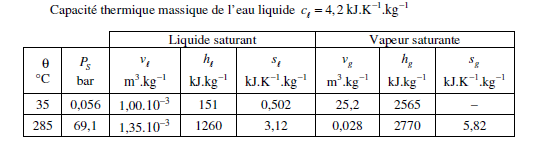
\includegraphics[width=\textwidth]{./Images/mp_s18_ex02.png}

\begin{enumerate}
	\item Représenter avec son sens le cycle décrit par l'eau dans le diagramme de Clapeyron $(P, v)$ et dans le diagramme des frigoristes $(\ln P, h)$. Qualifier chacune des cinq transformations par un ou plusieurs des qualificatifs suivants : isochore, isentropique, isobare, isotherme, adiabatique.
	\item Donner la valeur numérique des enthalpies massiques $h_A$, $h_C$, $h_D$ puis déterminer les entropies massiques $s_A$, $s_B$, $s_C$, $s_D$ et $s_E$.
	\item Calculer le titre en vapeur $x_E$ et l'enthalpie massique $h_E$.
	\item Calculer le transfert thermique massique reçu par le fluide dans le condenseur.
	\item On étudie la compression dans la pompe. On considère que le travail fourni par la pompe est négligeable devant les autres échanges énergétiques du cycle. En déduire $h_A = h_B$.
	\item Calculer le transfert thermique massique $q_{BD}$ fourni par le générateur de vapeur.
	\item Calculer le travail massique utile $w_u$ reçu par l'eau au cours du cycle.
	\item Sachant que la centrale développe une puissance de $\SI{900}{MW}$, calculer le débit massique du fluide dans le circuit.
	\item Quel est le rendement thermodynamique du cycle ? Le comparer au rendement de Carnot et commenter.
\end{enumerate}

\e{Réponses :}
\begin{enumerate}
	\item -
	\item hA = 151, hC = 1260, hD = 2770, sA = 0.502 = sB, sC = 3.12, sD = 5.82 = sE.
	\item xE = 0.68, hE = 1790.
	\item qEA = -1640
	\item qBD = 2620
	\item wu = -981
	\item Dm = 917 kg/s
	\item $\eta$=0.37 et carnot = 0.45	
\end{enumerate}

\subsection{Exercice 3 : Installation frigorifique}

On modélise le comportement thermodynamique du fluide dans une machine frigorifique à fluide diphasé par la succession de transformations suivantes :

\begin{itemize}
	\item Compression adiabatique réversible en phase gazeuse du point d'équilibre A au point d'équilibre B. En A, le fluide est à l'état de vapeur saturante.
	\item Refroidissement isobare de la vapeur de B en C. En C, le fluide est à l'état de vapeur saturante.
	\item Liquéfaction isobare et totale du fluide du point d'équilibre C au point d'équilibre D. Au point D, le fluide est à l'état de liquide saturant.
	\item Détente adiabatique irréversible du fluide que l'on peut ici modéliser par une détente isenthalpique entre D et E.
	\item Vaporisation totale isobare du fluide de E vers A.
\end{itemize}

On donne les enthalpies massiques du fluide aux points $A$, $B$ et $D$ : $$h_A = \SI{1167}{kJ\per\kilogram},~h_B = \SI{1355}{kJ\per\kilogram},~h_D = \SI{30}{kJ\per\kilogram}$$

\begin{enumerate}
	\item Représenter le cycle sur un diagramme de Clapeyron et un diagramme des frigoristes. Calculer les transferts thermiques $q_c$ et $q_f$ reçus par le fluide.
	\item Estimer le coefficient d'efficacité de la machine frigorifique.
	\item La phase gazeuse, de capacité thermique massique à pression constante $c_P$, peut être assimilée à un gaz parfait. Exprimer littéralement l'enthalpie massique de vaporisation $l_v(T_C)$ du fluide à la température au point C $T_C$ en fonction de $T_C$, $c_P$, $T_B$.
	\item Calculer numériquement le titre massique en vapeur $x_E$ sachant que l'enthalpie de vaporisation du fluide à la température $T_A$ est $l_v(T_A) = \SI{1293}{kJ\per\kilogram}$.
	\item On utilise cette installation frigorifique pour maintenir constante la température d'une chambre froide à laquelle il faut enlever $\SI{5000}{kJ}$ par heure. Calculer le débit massique $D_m$ du fluide frigorifique.
\end{enumerate}

\e{Réponses :}
\begin{enumerate}
	\item qc = -1325, qf = 1137
	\item eta = 6. Cela signifie qu'avec 1 J électrique fourni la machine peut ôter 6 J aux aliments à réfrigérer et donc évacuer 7 J dans l'air de la cuisine.
	\item hD-hB = -lv + cp(Tc-Tb)
	\item x = 0.12
	\item 1.22 g/s
\end{enumerate}
